Hier wird etwas sehr offensichtliches betrachtet. Dies passiert jedes Mal, wenn TF verwendet wird. 
Der Graph, der die Trainings- und Validationdaten nutzt, hat immer einen Einbruch in der Performanz an der Stelle an 
der TF gemacht wird. Dies ist in der Figure 3.3 deutlich bei Epoche zwanzig zu sehen.

\begin{figure}[htpb]
    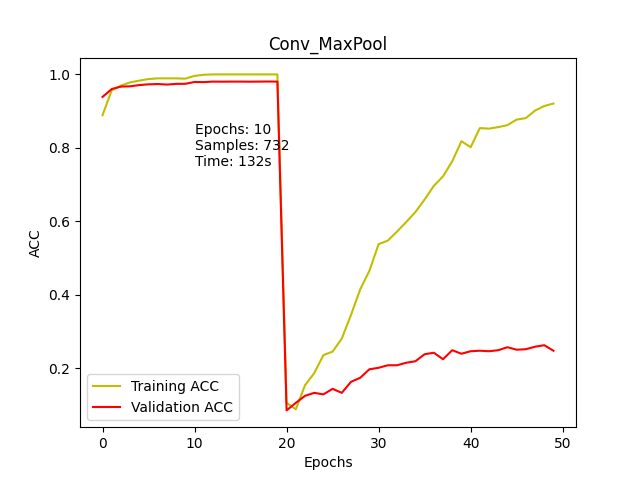
\includegraphics[height=5cm]{../../Plots/ba_plots/convmaxpool/convmaxpooltrain.png}
    \caption{\label{fig:convmaxpooltrain} Einbruch bei TF}
\end{figure}

Dieser Einbruch passiert jedes Mal nach TF. Dies liegt daran, dass das Netz bisher die Targetdaten noch nie gesehen hat und bisher 
auf eine andere Domain mit dem Sourcedatensatz trainiert hat. Das Netz kennt nur das Wissen aus dem Sourcedatensatz und kann nur dieses 
anwenden. Wenn man aber das Testset, welches nur über die Targetdaten geht auf das ganze Netzwerk betrachtet, kommt Figure 3.4 heraus. 

\begin{figure}[htpb]
    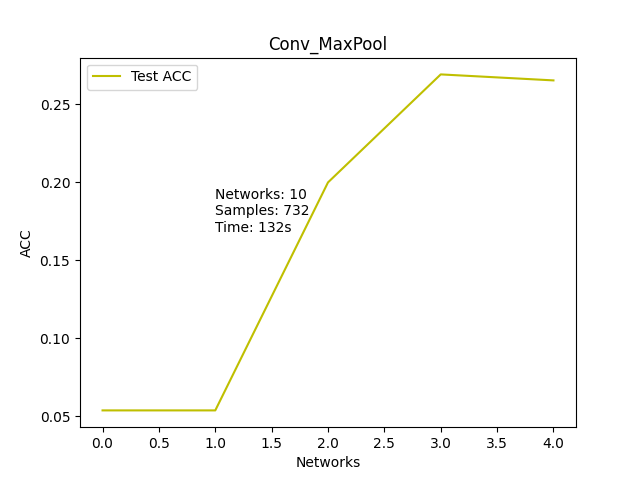
\includegraphics[height=5cm]{../../Plots/ba_plots/convmaxpool/convmaxpooltest.png}
    \caption{\label{fig:convmaxpooltest} Verbesserung auf Testdaten}
\end{figure}

Der Wechsel ist hierbei bei Netzwerk 2. Es ist eindeutig zu erkennen, dass es nach TF besser wird. Dies hat den Grund, dass das Netzwerk 
ab diesem Zeitpunkt auf den Trainingsdaten trainiert, die zum Testdatenset passen. 
